\homework{4}{Mon 17 Nov 2025 16:31}{}

\textbf{Problem 4.1.} Let $\mathcal{F}$ be a collection of affine functions. Prove that

\[
\phi(x)=\sup _{\ell \in \mathcal{F}} \ell(x)
\]

is a convex function.
\begin{proof}
	Take $x,y$ be points in the underlying linear space where $\phi$ and each $\ell$ is defined. Then for any $t \in (0,1)$ and any $\ell \in \mathcal{F}$ we have
	\begin{align*}
		t \phi(x) + (1 - t) \phi(y) \ge t \ell(x) + (1-t) \ell(y)
	.\end{align*}
	But since $\ell$ is affine, it respects linear combinations. Thus
	\[
		t \ell(x) + (1 - t) \ell(y) = \ell\left(t x + (1-t) y\right)
	.\] 
	Therefore
	\[
		t \phi(x) + (1 - t) \phi(y) \ge \ell\left(t x + (1-t) y\right)
	\] 
	for all $\ell \in \mathcal{F}$. Take the supremum on the right hand side, we have
	\[
		t \phi(x) + (1-t) \phi(y) \ge \phi\left(t x + (1-t) y\right)
	.\] 
	 Which says that $\phi$ is convex.
\end{proof}

\textbf{Problem 4.2.} For a Markov chain on 2 states with transition matrix
\[
\mathbf{P}=\left(\begin{array}{cc}
p & 1-p \\
1-p & p
\end{array}\right),
\]
do the following.\\
a) Compute an optimizer $u=\left(u_1, u_2\right)>0$ in the variational formula for the rate function $I_P(\mu)$ in Theorem IV.7.
Hint: The optimizer isn't unique since the function inside the braces in (IV.8) is unchanged if ( $u_1, u_2$ ) is replaced by ( $c u_1, c u_2$ ). Use this fact to reduce it to a onedimensional optimization problem.\\
b) Since $\mu_2=1-\mu_1$ we can view $I_P(\mu)$ as a function of $\mu_1$. Use your solution to part (a) and computer graphing software to plot $I_P\left(\mu_1, 1-\mu_1\right)$ for three different values of $p$ : $p=0.1, p=0.5$ and $p=0.75$.

\begin{proof}
	Theorem IV.7 gives us the following variational formula for $I_P(\mu)$ :
	\[
		I_P(\mu) =  \sup _{u > 0} \left( - \sum_{i=1}^{m} \mu_i \log \frac{(P u)_i}{u_i} \right) 
	.\] 
	We may take $\mu = (\mu_1, 1 - \mu_1)^T$ and $u = (1, r)$, since $\mu_1 + \mu_2 = 1$ and $u \mapsto cu$ for  $c \neq  0$ leaves the formula invariant. The formula becomes
	\[
		I_P(\mu) = 
		- \inf  _{r > 0} \left( \mu_1 \log \frac{p + (1-p) r}{1} + (1 - \mu_1) \log \frac{(1 - p) + pr }{r} \right) 
	.\] 
	Differentiate with respect to $r$, after rearrangement, this becomes
	\[
		\frac{\mu_1 (1 - p)}{p + (1 - p) r} + \frac{(1 - \mu_1) r (p-1) r^{-2}}{(1 - p) + pr}
	.\] 
	After simplification, we get a quadratic equation. This gives the quadratic solution
	\[
		r = \frac{\sqrt{(1 - p)^2 (2 \mu_1 - 1)^2 + 4 p^2 \mu_1 (1 - \mu_1)} - ( 1 - p) (2 \mu_1 - 1) }{2 p \mu_1}
	.\] 
	To check, if $\mu_1 = \frac{1}{2}, p = \frac{1}{2}$, this gives $r = 1$, so $u = (1, 1)^T$, consistent with the symmetry between the two dimensions.

	\begin{figure}
		\centering
		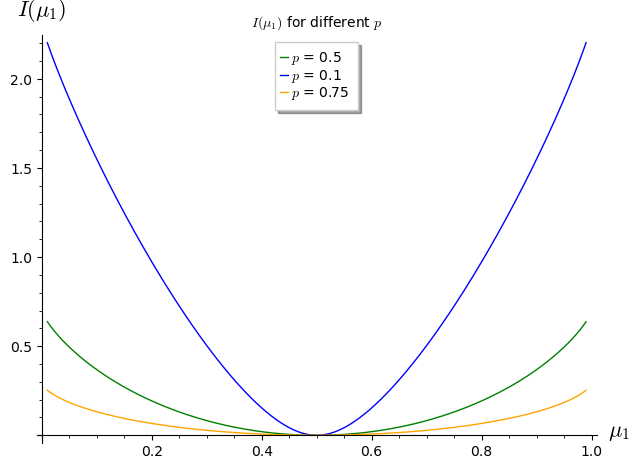
\includegraphics[width=0.7\textwidth]{figures/hw4.png}
		\caption{Plot of $I_P(\mu_1, 1 - \mu_1)$ for $p = 0.1, 0.5, 0.75$}
	\end{figure}

	Therefore, a feasible optimizer is
	\[
		(u_1, u_2) = (2 p \mu_1, \sqrt{(1 - p)^2 (2 \mu_1 - 1)^2 + 4 p^2 \mu_1 (1 - \mu_1)} - ( 1 - p) (2 \mu_1 - 1))
	.\] 

\end{proof}


\textbf{Problem 4.3.} Suppose that $X_1, X_2, X_3, \ldots$ are i.i.d. random variables and that $\{N(t)\}_{t \geq 0}$ is a homogeneous Poisson process with rate $\theta>0$ that is independent of the sequence $\left\{X_i\right\}_{i \geq 1}$, and let

\[
Z_n=\frac{1}{n} \sum_{i=1}^{N(n)} X_i .
\]


As motivation, think of the Poisson process modeling arrivals to a store (with time measured in days) and $X_i$ being the amount purchased by the $i$-th customer. Then $Z_n$ is the average amount purchased by customers per day in the first $n$ days.
a) Prove that

\[
\lim _{n \rightarrow \infty} \frac{1}{n} \log E\left[e^{n t Z_n}\right]
\]

exists and is finite whenever $\phi(t)=E\left[e^{t X_1}\right]$ is finite.\\
b) Prove that if the $X_i$ have bi- $\operatorname{Exp}(\mu)$ distribution (that is, they have p.d.f. $f(x)= \frac{\mu}{2} e^{-\mu|x|}$ ) then $Z_n$ satisfies a LDP.

\begin{proof}
	\begin{align*}
		E\left[ e^{n t Z_n} \right] 
		&= E\left[ e^{t \sum_{i=1}^{N(n)} X_i} \right] \\
		&= \sum_{k=0}^{\infty} E\left[ 1_{N(n) = k} e^{t \sum_{i=1}^{k} X_i} \right] \\
		&= \sum_{k=0}^{\infty} P(N(n) = k) \prod_{i=1}^{k} Ee^{t X_i}  \\
		&= \sum_{k=0}^{\infty} \frac{(\theta n)^k}{k!} e^{- \theta n} \phi(t)^k\\
		&= e^{\theta n \phi(t)} e^{- \theta n} 
	.\end{align*}
	Take the large deviation limit, we see that whenever $\phi(t) < \infty $,
	\[
		\frac{1}{n} \log E\left[ e^{n t Z_n} \right]
		= \frac{1}{n}(- \theta n (1 - \phi(t)))
		= - \theta + \theta \phi(t) < \infty 
	.\] 

	For bi-exponential  $X_i$, we compute $\varphi(t) = \int  e^{t x} \frac{\mu}{2}e^{- \mu |x|} dx = \frac{\mu}{2} (\int_{- \infty }^0 e^{(t + \mu)x}dx + \int _0^{\infty } e^{(t - \mu) x} dx )$, which is finite iff $t \in  (-\mu, \mu)$. When it is finite, we have $\varphi(t) = \frac{\mu}{2}\left( \frac{1}{t + \mu} - \frac{1}{t - \mu} \right) $.

	A bi-exponential distribution is well-defined only when $\mu > 0$ so we may assume so. Then we may compute
	\[
		\Lambda(t) = - \theta + \theta \varphi(t)
		= - \theta + \frac{\theta\mu}{2}\left( \frac{1}{t + \mu} - \frac{1}{t - \mu} \right)
	.\] 
	We see that $D_\Lambda = (-\mu, \mu)$ which contains $0$ in its interior. Therefore the assumptions for the Gärtner-Ellis theorem are satisfied and we may apply the first part of the theorem. To apply the second part of the theorem, we may observe from the formula of $\Lambda(t)$ that it is (1) continuous and blowing up at $t \to  \pm \mu$, hence l.s.c., (2) differentiale, on $D_\Lambda$. It only remains to verify that it is (3) steep. To this end, we compute the derivative,
	\[
F^{\prime}(t)=\frac{\theta \mu}{2}\left(\frac{1}{(t-\mu)^2}-\frac{1}{(t+\mu)^2}\right)
\]
We see that as $t \to -\mu$ or $t \to \mu$, the derivative blows up to infinity.

Therefore, both parts of the Gärtner-Ellis theorem apply and we obtain an LDP for $Z_n$.

\end{proof}

\textbf{Problem 4.4.} Suppose that $Y_1, Y_2, Y_3, \ldots$ are i.i.d. standard normal random variables, and let

\[
Z_n=\sum_{k=1}^n \frac{k}{n^2} Y_k^2 .
\]

a) Compute

\[
\Lambda(t)=\lim _{n \rightarrow \infty} \frac{1}{n} \log E\left[e^{n t Z_n}\right],
\]

and show that $\mathcal{D}_{\Lambda}=(-\infty, 1 / 2)$.\\
Hint 1: recall that $Y_1^2$ has chi-squared distribution, and thus $E\left[e^{t Y_1^2}\right]=\frac{1}{\sqrt{1-2 t}}$ for $t<\frac{1}{2}$.\\
Hint 2: identify the limit as a Riemann sum approximation.\\
b) Prove that $\Lambda(t)$ is not lower semi-continuous and that $\Lambda$ is not "steep" since $\lim _{t \rightarrow-\infty}\left|\Lambda^{\prime}(t)\right|<\infty$.\\
c) Prove that $Z_n$ satisfies a large deviation principle with rate function $\Lambda^*(x)$. Note: you cannot directly apply the 2nd half of the Gärtner-Ellis Theorem here since $\Lambda$ doesn't satisfy the necessary assumptions (this is the conclusion of part (b) above). However, you can prove that the set $E$ of exposed points of $\Lambda^*$ with exposing hyperplane in $\Lambda$ is the same as the set of points $\mathcal{D}_{\Lambda^*}=\left\{x: \Lambda^*(x)<\infty\right\}$ where $\Lambda^*$ is finite.

\begin{proof}
	Compute
	\begin{align*}
		E e^{n t Z_n}
		&= E e^{n t \sum_{k=1}^{n} \frac{k}{n^2}Y_k^2} \\
		&= E e^{\sum_{k=1}^{n} \frac{tk}{n}Y_k^2} \\
		&= \prod_{k=1}^{n} \frac{1}{\sqrt{1 - 2 \frac{t k}{n}} } 
	.\end{align*}
	Take $\frac{1}{n} \log $ to both sides,
	\begin{align*}
		\frac{1}{n} \log E e^{n t Z_n}
		&=\frac{1}{n} \sum_{k=1}^{n} \log \frac{1}{\sqrt{1 - 2 t \frac{k}{n}} }\\
		&\to \int _0^1 \log \frac{1}{\sqrt{1 - 2 t x} } dx\\
		&= -\frac{1}{2} \int _0^1 \log (1 - 2 t x) dx \\
		&= -\frac{1}{2}\left((1 - \frac{1}{2 t}) \log (1 - 2 t) - 1\right)
	.\end{align*}
	From the formula we see that $D_\Lambda = (- \infty , \frac{1}{2})$. Now compute its derivative:
	\[
		\Lambda' (t) = - \frac{2 t + \log (1 - 2 t)}{4 t^2}
	.\] 
	It blows up when $t \to \frac{1}{2}$, but goes to zero as $t \to  - \infty $. Hence $\Lambda$ is not steep. Looking at $\Lambda$, we see that $\Lambda$ is finite in a left-neighborhood of $\frac{1}{2}$ but not $t = \frac{1}{2}$, as $\log (1 - 2 t)$ is not defined at $t = \frac{1}{2}$. We also note that the limit as $t \to \frac{1}{2}^-$ is finite:
	\begin{align*}
		-\frac{1}{2} \left( (1 - \frac{1}{2t}) \log (1 - 2 t) - 1 \right) 
		&= \frac{1}{2}\frac{y}{1 - y} \log  y + \frac{1}{2} & y = 1 - 2 t \\
		&\to \frac{1}{2} & \text{as }y \to 0^+
	.\end{align*}
	This is because $y \log  y \to 0$ as $y \to 0$. Therefore, the function $\Lambda$ is not l.s.c. at $t = \frac{1}{2}$.

	Nevertheless, it still satisfies a large deviation principle. We can apply the first part of Gärtner-Ellis theorem. We have already verified that (1) $\Lambda(t)$ exist and (2) $0 \in \text{int} (D_\Lambda) = (- \infty , \frac{1}{2})$. So it has an LDP upper bound, and an LDP lower bound with open set $G$ replaced by $G \cap E$, where $E$ is the set of exposed points of $\Lambda^*$, where the exposing hyperplane is in $\text{int} (D_\Lambda)$.

	To verify that we indeed have an LDP lower bound, let's look at $\Lambda'(t)$. We see that this function is (1) continuously differentiable, (2) strictly monotone increasing, in its domain $D_\Lambda= (- \infty , \frac{1}{2})$. Hence, it has a continuously differentiable and strictly monotone increasing inverse, $g = (\Lambda')^{-1} : (0, + \infty ) \to (- \infty , \frac{1}{2})$. Then, we have that, the supremum in the definition of $\Lambda^*$ is attained at precisely $g(x)$ :

	\[
		\Lambda^*(x) 
		:= \sup_{t \in \mathbb{R}} x t - \Lambda(t) 
		= \sup_{t \in D_\Lambda} x t - \Lambda(t) 
		= x g(x) - \Lambda(g(x))
	.\] 
	Then, we see that $\Lambda^*$ is continuously differentiable. Now let's differentiate it as well:
	\[
		\Lambda^{*\prime}(x) = g(x) + x g'(x) - \Lambda'(g(x))g'(x)
	.\] 
	Use the fact that $g = (\Lambda')^{-1}$,
	\[
		\Lambda^{*\prime}(x) = g(x) + x g'(x) - x g'(x) = g(x)
	.\] 
	Then ${\Lambda^*}'' = g'(x) > 0$, so $\Lambda^*$ is strictly convex. Hence every point $x \in D_{\Lambda^*} = (0, + \infty )$ is an exposed point. Also, for every such $x$, the exposing hyperplane is ${\Lambda^*}'(x) = g(x) \in (- \infty , \frac{1}{2}) = D_{\Lambda}$. Hence, $E = D_{\Lambda^*}$. Therefore for every open $G \subset D_{\Lambda^*}$,  $G \cap E = G$, i.e. the LDP lower bound in the second half of Gärtner-Ellis theorem holds.

	


\end{proof}

